% Copyright (C) 2024 Yucheng Liu. Under the AGPL 3.0 License.
% AGPL 3.0 License: https://www.gnu.org/licenses/agpl-3.0.txt .

\section{Sample Figure}

\begin{figure}
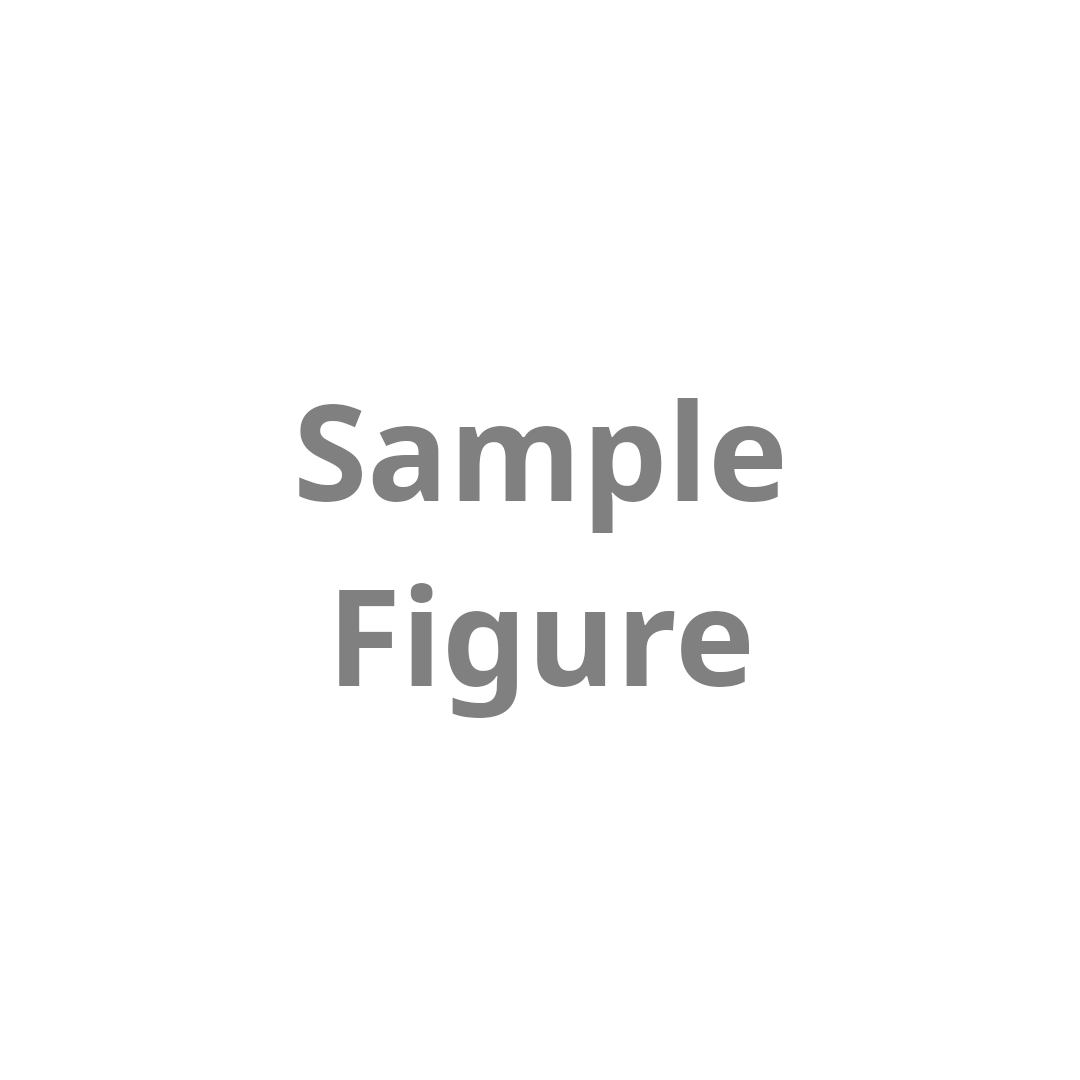
\includegraphics[width=\hsize]{./figures/figure_sample.png}
\caption{Sample figure.}
\label{figure_sample}
\end{figure}

Figure \ref{figure_sample} is a sample figure.

\section{Sideway Page}

Here is an example to have a page turned side way in the PDF. It is useful for having wide figures and tables in the thesis.

\begin{landscape} 
\begin{table}

\caption{
    Pearson's $\rho $ correlation of participated metrics with the WMT 2016 official average direct assessment human judgments on newstest 10k hybrid super-sampled systems at system level.
    Correlations of metrics not significantly outperformed by any other for that language pair are highlighted in bold.
}

\centering
\begin{tabular}{m{0.36\textwidth}cccccccc|cccccccc}
\hline & \multicolumn{8}{c|}{\textbf{into-English}} & \multicolumn{8}{c}{\textbf{out-of-English}} \\\textbf{Metric} & \textbf{cs} & \textbf{de} & \textbf{fi} & \textbf{lv} & \textbf{ru} & \textbf{tr} & \textbf{zh} & \textbf{avg.} & \textbf{cs} & \textbf{de} & \textbf{fi} & \textbf{lv} & \textbf{ru} & \textbf{tr} & \textbf{zh} & \textbf{avg.} \\ \hline
Blend  & .963 & \textbf{.969} & .956 & .976 & \textbf{.957} & .981 & .890 & .956 & -- & -- & -- & -- & .950 & -- & -- & -- \\ \hline
BEER & .966 & .952 & .954 & .974 & .930 & .969 & .897 & .949 & .963 & .829 & .975 & .923 & .942 & .968 & .906 & .929 \\ \hline
UHH\_TSKM & .990 & .929 & .918 & \textbf{.986} & .908 & .982  & .896  & .944  & --  & --  & --  & --  & --  & --  & --  & --  \\ \hline
CDER & .983  & .922  & .925  & .981  & .916  & .970  & \textbf{.898 } & .942  & .958  & .803  & .962  & .911  & .922  & .948  & \textbf{.975 } & .926  \\ \hline
TreeAggreg & .977  & .913  & \textbf{.975} & .983  & .912  & \textbf{.983 } & .854  & .942  & .942  & .765  & .963  & .915  & .919  & .971  & .933  & .915  \\ \hline
chrF++ & .935  & .957  & .924  & .970  & .938  & .957  & .876  & .937  & .966  & .835  & .977  & .944  & .942  & .975  & .968  & .944  \\ \hline
chrF & .933  & .960  & .935  & .965  & .946  & .941  & .855  & .934  & .968  & .845  & \textbf{.979 } & .945  & .947  & \textbf{.980 } & .969  & .947  \\ \hline
NIST & \textbf{.994} & .917  & .928  & .957  & .904  & .969  & .831  & .929  & .954  & .761  & .957  & .914  & .917  & .976  & .968  & .921  \\ \hline
TER & .983  & .899  & .950  & .967  & .905  & .951  & .837  & .927  & .951  & .790  & .959 & .888 & .930 & .958 & .965 & .920 \\ \hline
BLEU & .964  & .914  & .906  & .974  & .907  & .969  & .852  & .927  & .945  & .793  & .919  & .839  & .893  & .916  & .969  & .896  \\ \hline
MEANT-dvw.cos.wmax.n2.m.r8.$\alpha $1.0.$\beta $0.1 & .921  & .942  & .939  & .967  & .955  & .931  & .836  & .927  & --  & .844  & --  & --  & --  & --  & .944  & --  \\ \hline
CharacTER & .963  & .965  & .944  & .927  & .948  & .946  & .740  & .919  & \textbf{.973 } & \textbf{.893 } & .970  & .892  & .929  & .961  & .914  & .933 \\ \hline
WER & .981  & .889  & .946  & .965  & .900  & .922  & .828  & .919  & .949  & .797  & .959  & .884  & .931  & .947  & .951  & .917  \\ \hline
PER & .967  & .920  & .892  & .958  & .904  & .898  & .866  & .915  & .960  & .680  & .939  & .817  & .876  & .955  & .893  & .874  \\ \hline
MEANT-dvw.cos.wmax.n2.m.r8.$\alpha $1.0.$\beta $0.0 & .896  & .928  & .931  & .960  & .952  & .895  & .799  & .909  & .968  & .753  & .970  & \textbf{.947 } & \textbf{.955 } & .980  & .931  & .929  \\ \hline
AutoDA & .440  & .951  & .922  & .970  & .902  & .914  & .734  & .833  & .967  & .602  & .879  & .731  & .850  & .586  & .968  & .797  \\ \hline
\end{tabular}
\label{table_wmt17_sys}
\end{table}
\end{landscape} 
